% LaTeX template for Artifact Evaluation V20180201
%
% Prepared by Grigori Fursin (cTuning foundation, France and dividiti, UK)
% and Thierry Moreau (University of Washington, USA)
%
% This document was derived from the original Artifact Appendix
% prepared by Grigori Fursin (cTuning foundation, France and dividiti, UK) 
% and Bruce Childers (University of Pittsburgh, USA)
%
% See an example of this Artifact Appendix in the following CGO 2017 paper
% (with the artifact prepared using the Collective Knowledge framework):
% https://www.cl.cam.ac.uk/~sa614/papers/Software-Prefetching-CGO2017.pdf
%
% (C)opyright 2014-2018
%
% CC BY 4.0 license
%

\documentclass[sigconf]{acmart}

\usepackage{fancyvrb}
\DefineVerbatimEnvironment{verbatim}{Verbatim}{xleftmargin=.5in}

\newenvironment{packed_itemize}{
\begin{itemize}
  \setlength{\itemsep}{1pt}
  \setlength{\parskip}{0pt}
  \setlength{\parsep}{0pt}
}{\end{itemize}}

% DOI
\acmDOI{10.1145/3229762.3229766}

% ISBN
\acmISBN{978-1-4503-5923-8}

%Conference
\acmConference[ReQuEST at ASPLOS'18]{1st ACM Reproducible Quality-Efficient Systems Tournament on Co-designing Pareto-efficient Deep Learning}{March 2018}{Williamsburg, VA, USA}
\acmYear{2018}
\copyrightyear{2018}

%\acmPrice{15.00}

%\acmBadgeL[http://ctuning.org/ae/ppopp2016.html]{ae-logo}
%\acmBadgeR[http://ctuning.org/ae/ppopp2016.html]{ae-logo}


\begin{document}

\special{papersize=8.5in,11in}

\title{Leveraging the VTA-TVM Hardware-Software Stack \\for FPGA Acceleration of 8-bit ResNet-18 Inference}

\author{Thierry Moreau, Tianqi Chen, Luis Ceze}
\affiliation{University of Washington}

\renewcommand{\shortauthors}{}
\renewcommand{\shorttitle}{}

\maketitle

% \begin{abstract}
% \end{abstract}

\section{Extended Abstract}

We present a full-stack design to accelerate deep learning inference with FPGAs. Our contribution is two-fold. At the software layer, we leverage and extend TVM~\cite{chen:TVM}, the end-to-end deep learning optimizing compiler, in order to harness FPGA-based acceleration. At the the hardware layer, we present the Vanilla Tensor Accelerator (VTA) which presents a generic, modular, and customizable architecture for TPU-like accelerators.
Our results take a ResNet-18 description in MxNet and compiles it down to perform 8-bit inference on a 256-PE accelerator implemented on a low-cost Xilinx Zynq FPGA, clocked at 100MHz.
Our full hardware acceleration stack will be made available for the community to reproduce, and build upon\footnote{Available at: \url{http://github.com/uwsaml/vta}}.


\subsection{Technical Description}

Leveraging FPGA acceleration for deep learning workloads requires extensive cross-stack support.
Bridging the gap between a high-level and productivity-oriented neural network workload specification (MxNet, TensorFlow, PyTorch or Caffe2), and a low-level and efficiency-oriented executable tailored for hardware accelerators requires optimizations across multiple layers of the hardware-software stack.

\paragraph{High-Level Algorithm Specification}
We describe the ResNet-18 8-bit inference workload in MxNet~\cite{MXNet-whitepaper}, one of the mainstream deep learning frameworks.
MxNet produces an NNVM high-level graph representation of the workload.
Targeting deep learning hardware accelerators can impose constraints on the high-level graph representation, such as what sections of the inference graph are executing on the CPU or the FPGA, as well data layout constraints (e.g. tiling, spatial packing etc.).
Finally operators can be fused at the NNVM level in order to minimize data movement between memory and the FPGA.

\paragraph{Operator-Level Optimizations}
Next, each operator is specified, optimized and compiled for our deep learning accelerator using TVM~\cite{chen:TVM}.
TVM allows for separation between the algorithm specification (which is hardware agnostic) and the schedule optimizations (which differ for each hardware target).
Specifically, we utilize TVM's accelerator-specific schedule primitives to lower each graph operator into a sequence of operations that can execute on the FPGA-based accelerator. Those include:
\begin{itemize}
  \item Tensorization: convolutions and fully connected layers get lowered down to tensor operations, which execute efficiently in hardware (e.g. single-cycle matrix-matrix multiplication as in ~\cite{Jouppi:TPU}).
  \item Virtual Threading: virtual threads are exposed in order to present two concurrent execution threads that execute on mutually exclusive data partitions to keep compute and memory resources busy as much as possible (e.g. decoupled access-execute as in ~\cite{Smith:DAE} to maximize resource utilization).
  \item Memory Scoping: TVM can explicitly manage accelerator memory resources by assigning local data buffers to a specific scope that corresponds to an SRAM structure on the FPGA accelerator.
\end{itemize}

\paragraph{Runtime and JIT Compilation}
After the TVM optimization and lowering phases, we obtain a lowered LLVM-compilable program with calls into the accelerator's runtime.
The runtime assembles the accelerator instruction stream and micro-kernels on the fly in JIT fashion.
This offloads the complexities of generating assembly away from the TVM stack.
The runtime also handles synchronization between the CPU and the FPGA when computation is being offloaded onto the accelerator.

\begin{figure}[t]
\centering
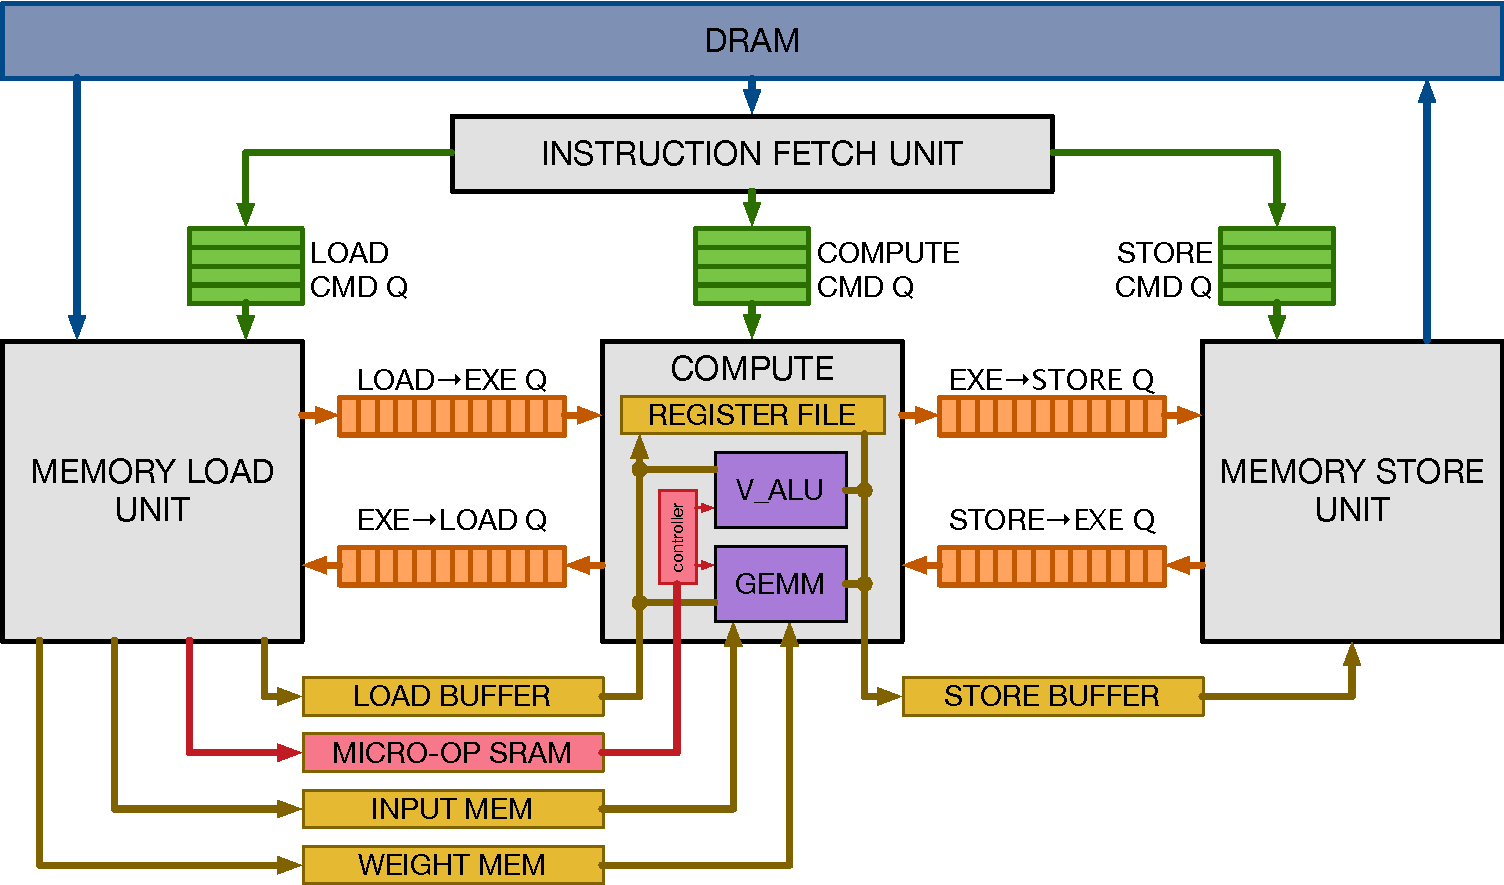
\includegraphics[width=0.8\columnwidth]{figures/vta_overview}
\caption{VTA Hardware Design Overview.}
\label{fig:vta_overview}
\end{figure}

\paragraph{Versatile Tensor Accelerator (VTA)}
We provide an overview of VTA: a generic, modular and customizable TPU-like hardware accelerator design.
At its core, the VTA design can perform a single matrix-matrix multiplication per cycle.
These \emph{tensorized} operations are tailored to take advantage of the high operational intensity of deep learning workloads.
VTA is programmed with CISC instructions that describe high-level, multi-cycle tensor operations, and RISC micro-kernel instructions that dictate low-level data access patterns for CISC compute-instructions.
In order to maximize compute resources utilization, VTA relies on a decoupled access-execute pipeline~\cite{Smith:DAE} where memory loads, memory stores, and computation can occur independently, and concurrently.
We show a high-level schematic of the VTA design in Figure~\ref{fig:vta_overview}: each pipeline stage communicates via dependence queues that guarantee correctness of execution.
Those dependence queues are explicitly programmed via synchronization operations that are added to the instruction stream in the JIT compilation phase.
These synchronization operations are derived from thread context information which TVM produces when the user parallelizes a workload across two virtual threads.
This virtual thread lowering process is described in more depth in ~\cite{chen:TVM}.

\subsection{Empirical Evaluation}

We train a ResNet-18 neural network with MxNet, and perform post-training tuning on the parameters to convert them to 8-bit weights from 32-bit floating point.
The Imagenet top-5 validation accuracy is 63\% after fixed-point conversion.

We implement the VTA design on a low-power PYNQ board which incorporates an ARM Cortex A9 dual core CPU clocked at 667MHz and an Artix-7 based FPGA fabric.
On the modest FPGA resources, we implement a $16\times16$ matrix-vector unit clocked at 100MHz that performs products of 8-bit values and accumulates them into a 32-bit register every cycle.
The theoretical peak throughput of this flavor of the VTA design lies around 51GOPS/s.
We allocate 16kB of resources for microkernel cache, 32kB of resources for activation storage, 256kB for parameter storage, and 128kB for the register file (i.e. accumulator storage).
These on-chip buffers are nowhere near large enough to provide enough on-chip storage for a single layer of ResNet, and therefore provide motivational case-study for effective memory reuse and memory access latency hiding.

We offload all convolution layers of the ResNet-18 network onto the FPGA accelerator, except for the first convolution layer C1, which is evaluated on the CPU due to its low number of input channels.
Activations and batch normalization operators are evaluated on the FPGA, while max pooling and fully connected layers are evaluated on the CPU.

We describe each of the ResNet-18 layers that we evaluated on the FPGA in Table~\ref{table:resnet18}.

\begin{table}[t]
  \begin{footnotesize}
	\begin{tabular}{ccccc}
	\hline
	Name & Operator & $H, W$ & $IC, OC$ & $K, S$ \\
	\hline
	C1  & conv2d & 224, 224 & 3,64  & 7, 2 \\
	C2  & conv2d & 56, 56 & 64,64   & 3, 1 \\
	C3  & conv2d & 56, 56 & 64,64   & 1, 1 \\
	C4  & conv2d & 56, 56 & 64,128  & 3, 2 \\
	C5  & conv2d & 56, 56 & 64,128  & 1, 2 \\
	C6  & conv2d & 28, 28 & 128,128 & 3, 1 \\
	C7  & conv2d & 28, 28 & 128,256 & 3, 2 \\
	C8  & conv2d & 28, 28 & 128,256 & 1, 2 \\
	C9  & conv2d & 14, 14 & 256,256 & 3, 1 \\
	C10 & conv2d & 14, 14 & 256,512 & 3, 2 \\
	C11 & conv2d & 14, 14 & 256,512 & 1, 2 \\
	C12 & conv2d &  7,  7 & 512,512 & 3, 1 \\
	\hline
	\end{tabular}
  \end{footnotesize}
	\centering
	\caption{\small{Configurations of all conv2d operators in ResNet-18 used in the single kernel experiment.
	H/W denotes height and width, IC input channels, OC output channels,
	K kernel size, and S stride size. All ops use ``SAME'' padding.}}
	\label{table:resnet18}
\end{table}

\begin{figure}[!t]
\centering
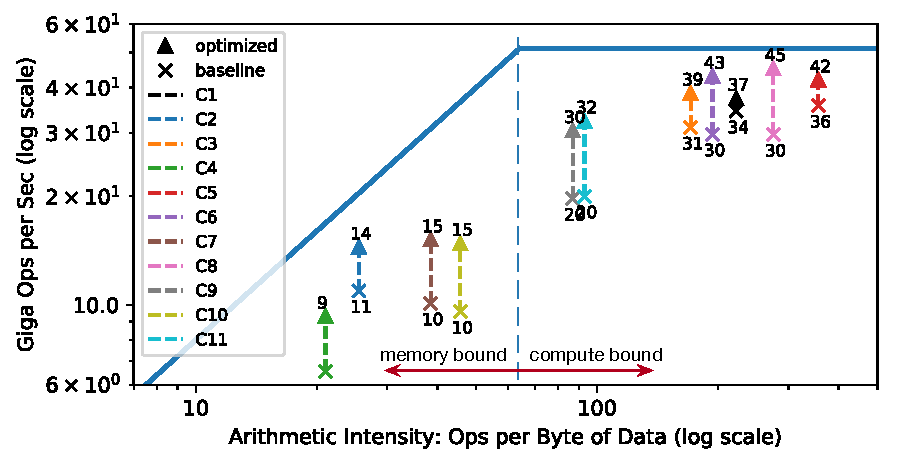
\includegraphics[width=0.9\columnwidth]{figures/vta_roofline}
\caption{\small{Roofline of an FPGA-based deep learning accelerator running ResNet inference. With latency hiding enabled by TVM, the performance of the benchmarks are brought closer to the roofline, demonstrating higher compute and memory bandwidth efficiency.}}
\label{fig:fpga_latencyhiding}
\end{figure}

\paragraph{Single Kernel Evaluation}
We evaluate each layer individually to evaluate TVM's ability to efficiently utilize the accelerator's resources.
The results are shown in the Roofline diagram in Figure ~\ref{fig:fpga_latencyhiding}.
Roofline performance diagrams provide insight on how well computation and memory resources are utilized on a given system for different workloads.
Overall, virtual threading in TVM improves performance on all ResNet layers by exploiting latency hiding mechanisms in VTA's decoupled access-execute pipeline.
Peak compute utilization increases from 70\% with no virtual threading to 88\% with virtual threading turned on (to hide memory access latency).

\paragraph{End-to-end ResNet Evaluation}
We leverage TVM to generate ResNet inference kernels on the PYNQ platform and offload as many layers as possible to VTA.
We utilize TVM to generate both schedules for the CPU only and CPU+FPGA implementation.
Due to its shallow convolution depth, the first ResNet convolution layer could not be efficiently offloaded on the FPGA and is instead computed on the CPU.
All other convolution layers in ResNet, however, are amenable to efficient offloading.
Operations including residual layers and max pooling are also performed on the CPU since our TVM extensions do not support these operations yet.

\begin{figure}[t]
\centering
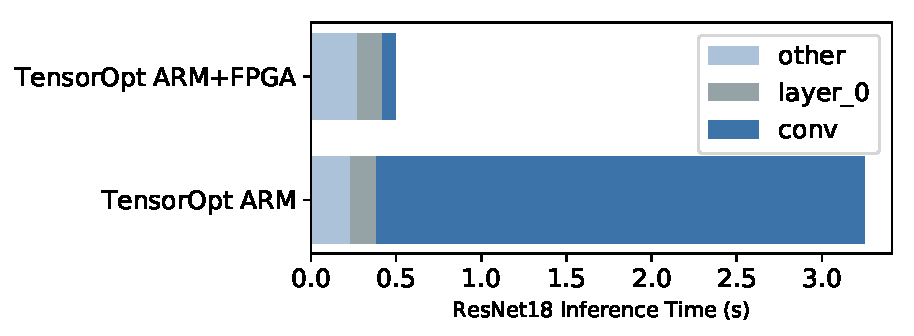
\includegraphics[width=0.9\columnwidth]{figures/exp_fpga_e2e}
\caption{\small{We offload convolutions in the ResNet workload to an FPGA-based accelerator.
The grayed-out bars correspond to layers that cannot be accelerated by the FPGA and therefore have to run on the CPU. The FPGA can provide a 40x acceleration on offloaded convolution layers over the Cortex A9.}}
\label{fig:e2e_fpga}
\end{figure}

\bibliographystyle{ACM-Reference-Format}
\bibliography{paper}

\newpage

\onecolumn

\appendix
\section{Artifact Appendix}

Submission and reviewing methodology: \\
{\em http://cTuning.org/ae/submission-20171101.html}

%%%%%%%%%%%%%%%%%%%%%%%%%%%%%%%%%%%%%%%%%%%%%%%%%%%%%%%%%%%%%%%%%%%%%
\subsection{Abstract}

This Artifact Appendix describes the experimental workflow,
artifacts and results from this paper evaluated 
during the 1st reproducibility-focused ReQuEST tournament at the ACM ASPLOS'18:

\begin{packed_itemize}
  \item {\bf Original artifact:} \url{https://github.com/uwsaml/vta}
  \item {\bf Latest CK workflow:} \url{https://github.com/ctuning/ck-request-asplos18-resnet-tvm-fpga}
  \item {\bf CK results:} \url{https://github.com/ctuning/ck-request-asplos18-results-resnet-tvm-fpga}
  \item {\bf Artifact DOI:} \url{https://doi.org/10.1145/3229772}
  \item {\bf ReQuEST submission and reviewing guidelines:} \url{http://cknowledge.org/request-cfp-asplos2018.html} (\cite{request-asplos18})
  \item {\bf ReQuEST goals:} \cite{cm:29db2248aba45e59:0c7348dfbadd5b95}
  \item {\bf ReQuEST workflows:} \url{https://github.com/ctuning/ck-request-asplos18-results}
  \item {\bf ReQuEST scoreboard:} \url{http://cKnowledge.org/request-results}
\end{packed_itemize}

Our original hardware and software artifact is fully contained under: \url{https://github.com/uwsaml/vta}.
Our repository contains README.md instructions on how to deploy, and reproduce the software and hardware artifacts on the Pynq FPGA development platform.

%%%%%%%%%%%%%%%%%%%%%%%%%%%%%%%%%%%%%%%%%%%%%%%%%%%%%%%%%%%%%%%%%%%%%
\subsection{Artifact check-list}

Details: \url{http://cTuning.org/ae/submission_extra.html}

\begin{itemize}
  \item {\bf Algorithm:} Deep Learning, Neural Networks, ResNet-18 inference, 2D convolution.
  \item {\bf Program:} MxNet.
  \item {\bf Compilation:} NNVM, TVM.
  \item {\bf Transformations:} TVM schedule optimizations include: loop splitting, loop reordering, tensorization, virtual threading. Neural network optimizations include: quantization, operator fusion.
  \item {\bf Binary:} FPGA bitstream and RPC server executable.
  \item {\bf Data set:} ImageNet 2012 validation (50,000 images) and ResNet-18 8-bit.
  \item {\bf Run-time environment:} Ubuntu 15.04; Python2/3.
  \item {\bf Hardware:} Xilinx Pynq-Z1 FPGA development board, x86 host machine.
  \item {\bf Run-time state:} 667MHz CPU clock, 100MHz FPGA clock, 2W SoC peak consumption.
  \item {\bf Execution:} Remote execution via RPC.
  \item {\bf Metrics:} Total execution time; top1/top5 accuracy over some (all) images from the data set.
  \item {\bf Output:} Classification result; execution time; accuracy.
  \item {\bf Experiments:} Automated via CK command line.
  \item {\bf How much disk space required (approximately)?:} 200MB for VTA repository and dependences after compilation.
  \item {\bf How much time is needed to prepare workflow (approximately)?:} 15 mins for inference only, 2 hours for re-compilation of FPGA hardware artifact.
  \item {\bf How much time is needed to complete experiments (approximately)?:} 20 mins for full Imagenet test dataset.
  \item {\bf Publicly available?:} Will be (not at the time of the publishing).
  \item {\bf Code license?:} Apache 2.0.
  \item {\bf Collective Knowledge workflow framework used?:} Yes.
  \item {\bf CK workflow URL:} \url{https://github.com/ctuning/ck-request-asplos18-resnet-tvm-fpga}
  \item {\bf CK results URL:} \url{https://github.com/ctuning/ck-request-asplos18-results-resnet-tvm-fpga}
  \item {\bf Original artifact URL:} \url{https://github.com/uwsaml/vta}
\end{itemize}

%%%%%%%%%%%%%%%%%%%%%%%%%%%%%%%%%%%%%%%%%%%%%%%%%%%%%%%%%%%%%%%%%%%%%
\subsection{Description}

\subsubsection{How to obtain}

Our artifact is fully contained under: \url{https://github.com/uwsaml/vta}.
Our repository contains instructions on how to deploy, and reproduce the software and hardware artifacts on the Pynq FPGA development platform.

\subsubsection{Hardware dependencies}

Reproducing the hardware artifact requires a Pynq development board (\url{http://www.pynq.io/}) along with a power supply, an 8+GB SD card, and an Ethernet cable to communicate with the host.
In order to run the example, any x86 machine should do.
Compiling the hardware requires a machine with at least 4GB of RAM, two cores, and 30GB of disk space for the Xilinx Vivado FPGA toolchains.

\subsubsection{Software dependencies}

Reproducing the examples requires Python, Numpy, MxNet, NNVM (\url{nnvm.tvmlang.org}) and TVM  (\url{tvm.ai}) installed. We describe the installation process in the VTA Github repo README files.

\subsubsection{Data sets}

We provide cached pre-trained network parameters, and a pre-compiled bitstreams to be downloaded from self-hosted servers.
The ImageNet dataset can be accessed on the official website: \url{http://www.image-net.org/}.

%%%%%%%%%%%%%%%%%%%%%%%%%%%%%%%%%%%%%%%%%%%%%%%%%%%%%%%%%%%%%%%%%%%%%
\subsection{Installation}

The installation instructions are detailed under: \url{https://github.com/uwsaml/vta}.

%%%%%%%%%%%%%%%%%%%%%%%%%%%%%%%%%%%%%%%%%%%%%%%%%%%%%%%%%%%%%%%%%%%%%
\subsection{Experiment workflow}

The experimental workflow was ported to utilize CK under \url{https://github.com/ctuning/ck-request-asplos18-resnet-tvm-fpga}.

%%%%%%%%%%%%%%%%%%%%%%%%%%%%%%%%%%%%%%%%%%%%%%%%%%%%%%%%%%%%%%%%%%%%%
\subsection{Evaluation and expected result}
We describe the experimental metrics of our artifact below:
\begin{itemize}
\item Single batch inference time: 0.42s.
\item Top-1 accuracy: 37\%.
\item Top-5 accuracy: 63\%.
\item Power consumption: peak 2W for SoC.
\item Device cost: \$65 for academics (at the time of the paper submission), \$200 otherwise.
\end{itemize}

%%%%%%%%%%%%%%%%%%%%%%%%%%%%%%%%%%%%%%%%%%%%%%%%%%%%%%%%%%%%%%%%%%%%%
% \subsection{Experiment customization}

%%%%%%%%%%%%%%%%%%%%%%%%%%%%%%%%%%%%%%%%%%%%%%%%%%%%%%%%%%%%%%%%%%%%%
% \subsection{Notes}

%%%%%%%%%%%%%%%%%%%%%%%%%%%%%%%%%%%%%%%%%%%%%%%%%%%%%%%%%%%%%%%%%%%%%
\subsection{Unified installation and evaluation for the ReQuEST scoreboard using Collective Knowledge framework}

\subsubsection{Minimal CK installation}

The minimal installation requires:

\begin{packed_itemize}
 \item Python 2.7 or 3.3+ (limitation is mainly due to unitests)
 \item Git command line client.
\end{packed_itemize}

You can install CK in your local user space as follows:

\begin{verbatim}
$ git clone http://github.com/ctuning/ck
$ export PATH=$PWD/ck/bin:$PATH
$ export PYTHONPATH=$PWD/ck:$PYTHONPATH
\end{verbatim}

You can also install CK via PIP with sudo to avoid setting up environment variables yourself:

\begin{verbatim}
$ sudo pip install ck
\end{verbatim}

\subsubsection{CK repository installation}

\begin{verbatim}
$ ck pull repo:ck-request-asplos18-resnet-tvm-fpga
\end{verbatim}

\subsubsection{Install this CK workflow from the ACM Digital Library snapshot}

It is possible to install and test the snapshot of this workflow 
from the ACM Digital Library without interfering with your current CK installation.
Download related file "request-asplos18-artifact-?-ck-workflow.zip"
to a temporary directory, unzip it and then execute the following commands:

\begin{verbatim}
$ . ./prepare_virtual_ck.sh
$ . ./start_virtual_ck.sh
\end{verbatim}

All CK repositories will be installed in your current directory.
You can now proceed with further evaluation as described below.

\subsubsection{PYNQ-Z1 FPGA installation (connected via RPC from host)}

Please follow this getting-started guide (\url{https://github.com/uwsaml/vta/tree/master/apps/pynq_rpc}) to set up your Pynq board.

We used pynq\_z1\_image\_2017\_02\_10.img with 16GB microSD card and Ubuntu 15.04.

Turn on your board. You should now be able to connect to it as follows:

\begin{verbatim}
$ ssh xilinx@192.168.2.99
\end{verbatim}

Use 'xilinx' as password (unless you changed it).

\textbf{Install global prerequisites (Ubuntu)}

Note that Ubuntu 15.04 is now outdated. You need to fix URLs of Ubuntu repos to be able to update it and install missing packages as follows:

\begin{verbatim}
$ sudo vim /etc/apt/sources.list.d/multistrap-wily.list
 deb [arch=armhf] http://old-releases.ubuntu.com/ubuntu wily universe main
 deb-src http://old-releases.ubuntu.com/ubuntu wily universe main
\end{verbatim}

Then you should be able to upgrade your distribution as follows:

\begin{verbatim}
$ sudo apt update
$ sudo apt upgrade
\end{verbatim}

Now you can install missing deps:

\begin{verbatim}
$ sudo apt install python-pip python3-pip
$ pip install wget
\end{verbatim}

\textbf{Install Collective Knowledge and this repository with all dependencies}

\begin{verbatim}
$ sudo pip install ck
$ ck pull repo:ck-request-asplos18-resnet-tvm-fpga
\end{verbatim}

\textbf{Install and run VTA RPC server via CK}

\begin{verbatim}
$ ck install package:lib-tvm-runtime-master \
   --env.PACKAGE_GIT_CHECKOUT=e4c2af9abdcb3c7aabafba8084414d7739c17c4c
\end{verbatim}

Choose Python 3!

\begin{verbatim}
$ ck run program:vta-pynq-server --sudo
\end{verbatim}

During first execution other missing soft dependencies 
will be detected or installed including libdma.so and VTA server.

If libdma.so is installed in an unusual directory and was not automatically found by CK, 
you can register it manually as follows (and then restart above commands):

\begin{verbatim}
$ ck detect soft:lib.pynq.dma --search_dirs={path to libdma.so)
\end{verbatim}

Note that by default this server will run on host '192.168.2.99' and port '9091'.

Now you can configure your host machine to classify images via this board.

\subsubsection{Installation: host machine (tested on Ubuntu or similar)}

Install missing deps:

\begin{verbatim}
$ sudo apt install python-pip python3-pip
$ pip install wget
\end{verbatim}

\textbf{Install Collective Knowledge and this repository with all dependencies}

\begin{verbatim}
$ sudo pip install ck
$ ck pull repo:ck-request-asplos18-resnet-tvm-fpga
\end{verbatim}

\textbf{Install TVM, NNVM and VTA}

\begin{verbatim}
$ ck install package:lib-tvm-master-cpu \
   --env.PACKAGE_GIT_CHECKOUT=e4c2af9abdcb3c7aabafba8084414d7739c17c4c
\end{verbatim}

Select Python 2.x and LLVM > 4.x

\begin{verbatim}
$ ck install package:lib-nnvm-master --env.PACKAGE_URL=https://github.com/tqchen/nnvm \
    --env.PACKAGE_GIT_CHECKOUT=qt
$ ck install package:lib-vta-python-master
\end{verbatim}

\textbf{Set up RPC access to VTA server}

\begin{verbatim}
$ ck add machine:pynq
\end{verbatim}

Select "remote machine accessed via RPC", then enter hostname and port.

You can then check if VTA server running as follows:

\begin{verbatim}
$ ck show machine
\end{verbatim}

\textbf{Run classification}

You can now try to classify some image via VTA server as follows:

\begin{verbatim}
$ ck run program:request-tvm-vta-pynq --cmd_key=classify --target=pynq
\end{verbatim}

\textbf{Test accuracy}

Finally, you can test accuracy on IMAGENET as follows:

\begin{verbatim}
$ ck run program:request-tvm-vta-pynq --cmd_key=test target=pynq
\end{verbatim}

Note that if board crahes, you can restart above program and it will continue aggregating statistics
via "program/request-tvm-vta-pynq/tmp/aggregate-ck-timer.json" file. 
You can delete it if you want to collect "fresh" stats.

\textbf{Run benchmarking in a unified ReQuEST way and record results}

You can run performance benchmark and record experiments as follows:

\begin{verbatim}
$ cd `ck find script:benchmark-request-tvm-fpga`
$ python benchmarking.py
\end{verbatim}

Your results will be recorded in local:experiment:ck-request-asplos18-tvm-fpga-performance-* entries:
\begin{verbatim}
$ ck ls local:experiment:ck-request-asplos18-tvm-fpga-performance-*
\end{verbatim}

You can pack them and send to ReQuEST organizers as follows:

\begin{verbatim}
$ ck zip local:experiment:ck-request-asplos18-tvm-fpga-performance-*
\end{verbatim}

\end{document}
